\documentclass[graphics]{beamer}
\usepackage{xcolor}
\usepackage{graphicx}
\usepackage{verbatim}
\usepackage{wrapfig}
\usepackage{tabularx}
\usepackage{multirow}
\usepackage{amssymb}
\usepackage{pifont}
\usepackage{tikz}
\def\Checkmark{\tikz\fill[scale=0.2](0,.35) -- (.25,0) -- (1,.7) -- (.25,.15) -- cycle;} 

\useoutertheme{shadow}
%\usecolortheme{orchid}
\usecolortheme{seahorse}
\newcommand{\cmark}{\text{\ding{51}}}
%\newcommand*{\GtrSim}{\smallrel\gtrsim}

% math commands
\newcommand{\be}{\begin{eqnarray}}
\newcommand{\ee}{\end{eqnarray}}
\newcommand{\beq}{\begin{equation}}
\newcommand{\eeq}{\end{equation}}
\def\simless{\mathbin{\lower 3pt\hbox
      {$\rlap{\raise 5pt\hbox{$\char'074$}}\mathchar"7218$}}}
\def\simgreat{\mathbin{\lower 3pt\hbox
      {$\rlap{\raise 5pt\hbox{$\char'076$}}\mathchar"7218$}}} %> or of order

% variables

\def\toonscale{0.45}
\def\mboxy#1{\mbox{\small #1}}

\defbeamertemplate*{title page}{customized}[1][]
{
  \usebeamerfont{title}\inserttitle\par
  \usebeamerfont{subtitle}\usebeamercolor[fg]{subtitle}\insertsubtitle\par
  \bigskip
  \usebeamerfont{author}\insertauthor\par
  \usebeamerfont{institute}\insertinstitute\par
  \usebeamerfont{date}\insertdate\par
  \usebeamercolor[fg]{titlegraphic}\inserttitlegraphic
}
\begin{comment}
\AtBeginSection[]{
  \frame{
    \frametitle{Outline}
    \tableofcontents[currentsection]
  }
}
\end{comment}


\title{\textcolor{red}{Lunar view of pulsars and ISM}}
%\subtitle{}
\author[U. Pen]{{
{ 
}, 
\textcolor{red}{\small 
  Ue-Li Pen} 
}
\\[8mm] 
}
\date{\textcolor{blue}{January 24, 2019}}


\begin{document}


%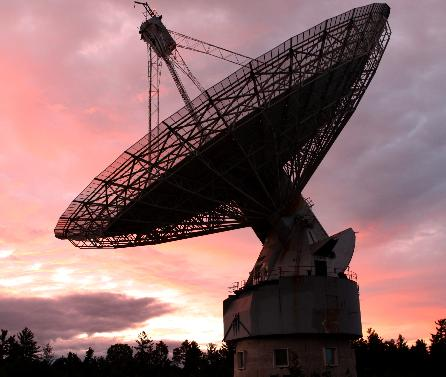
\includegraphics[width=4.4in]{Figures/IMG-7749-ARO-crop.JPG}

\frame{
\vspace{-0.5in}
\begin{center}  
%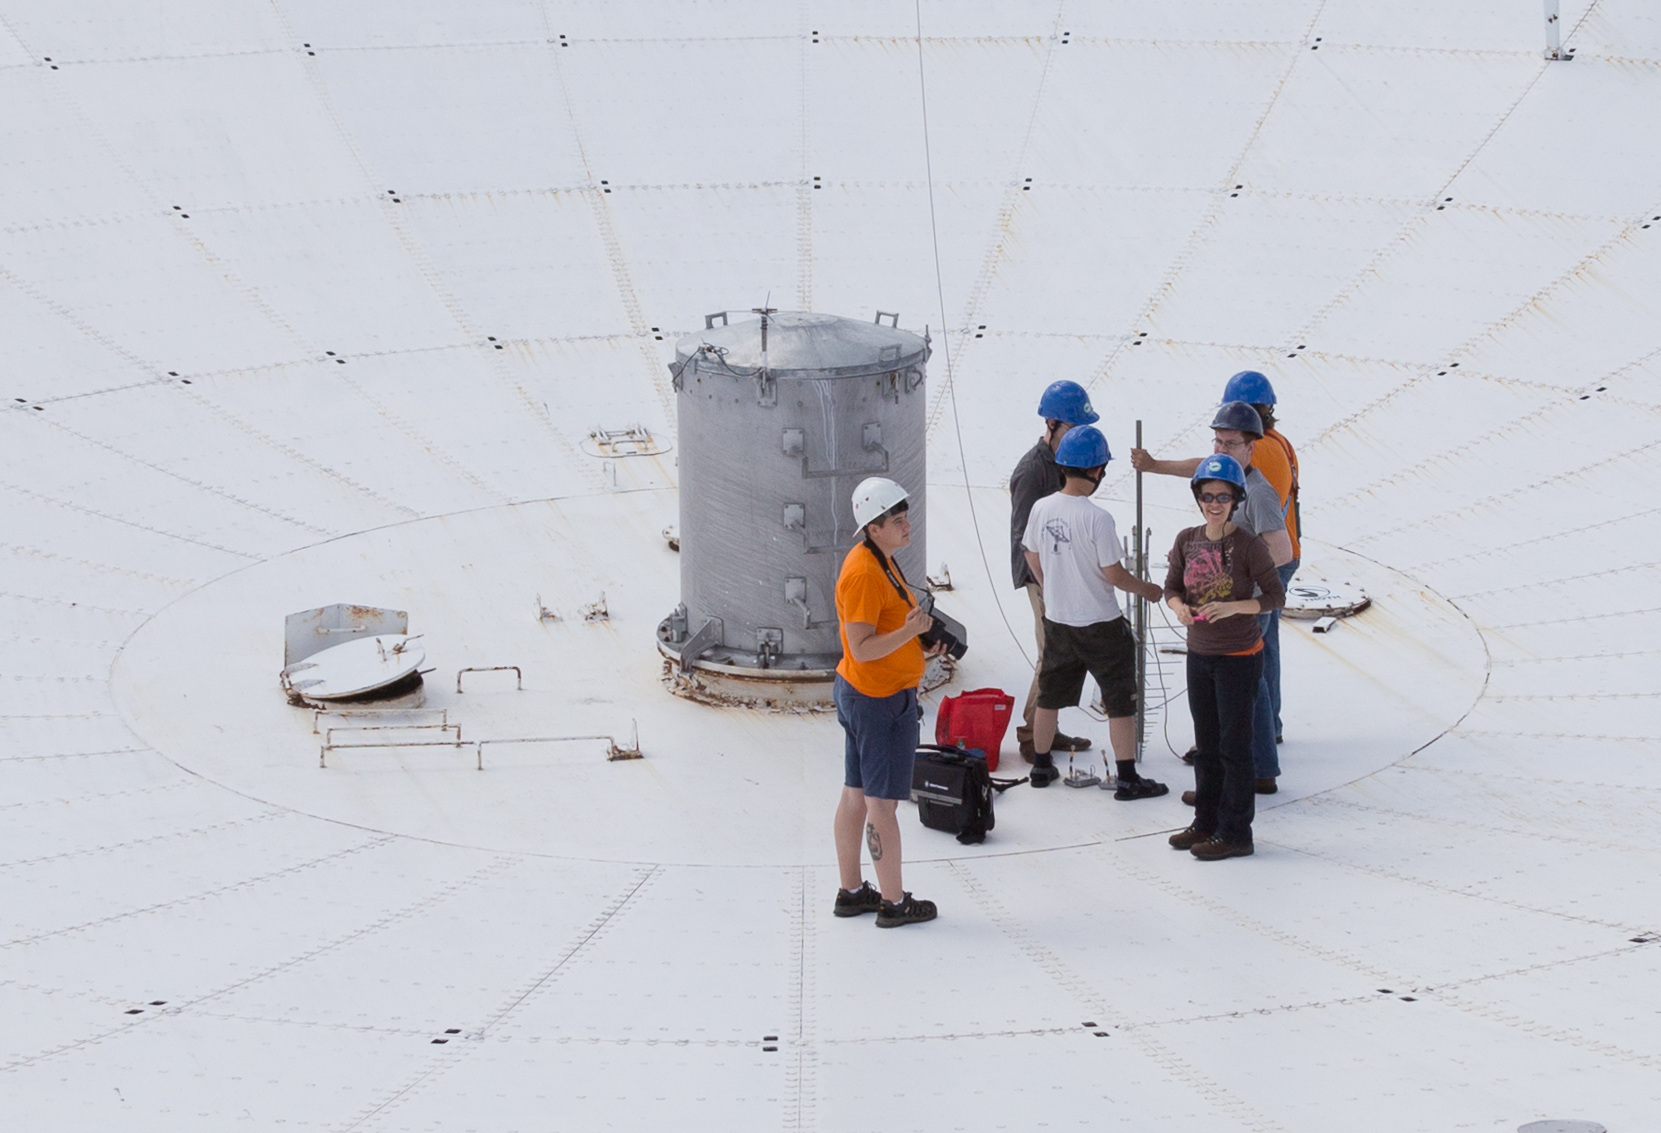
\includegraphics[width=4.4in]{Figures/IMG-0438-by-Andre-cropped.jpg}
\end{center}
\begin{picture}(320,250)
\put(-50,60){
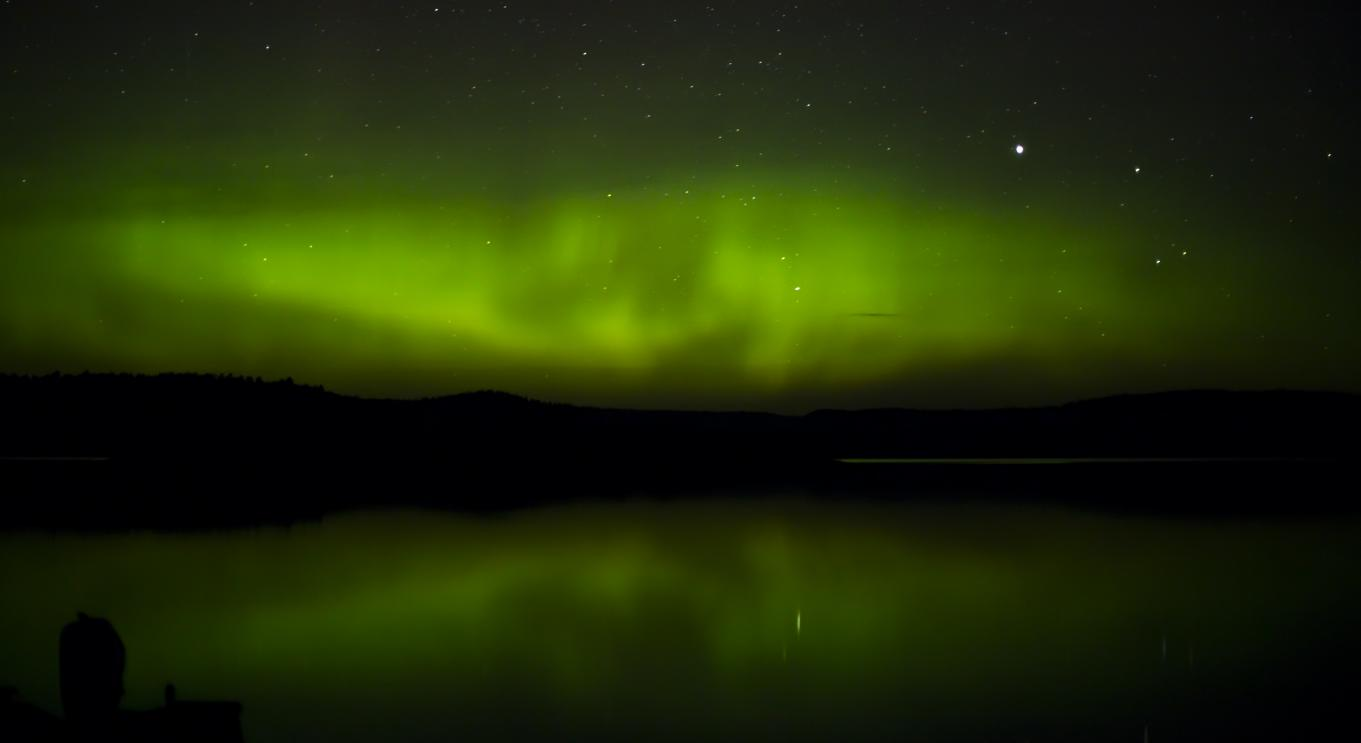
\includegraphics[width=5.5in]{Figures/traverse-aurora.jpg}}
\end{picture}
\vspace{-4in}
\\
image credit: Andre Recnik
\\
\vspace{1in}
\titlepage
}


%\section*{Introduction}
\section{Introduction}

\begin{comment}
  \subsection{Outline}

  \frame{
    \frametitle{Outline}
    \tableofcontents
  }
\end{comment}

  \frame{
    \frametitle{Overview}
    \begin{itemize}
      \item Moon: unique frequency, position
      \item access to lower frequencies
      \item VLBI to Earth
      \end{itemize}
  }


  \frame{
    \frametitle{Low Frequency}
    \begin{itemize}
      \item pulsar emission mechanism not understood
      \item generally steep spectral index: most energy emitted at low
        frequency, for some pulsars cutoff is unknown
      \item some cutoff in observable band, some keep rising
      \item observations below ionospheric cutoff
    \end{itemize}
  }


\frame{
    \frametitle{VLBI}
    \begin{itemize}
      \item Pulsar radiation is coherent: like Laser, RADAR
      \item forms interference pattern: strong scintillation/scattering
      \item effect strongest at low frequencies
      \item observations on earth and at far location allows
        construction of propagation screen
      \item Brisken et al 2010, Simard and Pen 2018
      \item most lenses not resolved with Earth baselines
      \item bigger effect at lower frequencies, longer baselines
      \item some exploratory data from RadioAstron        
    \end{itemize}
}



\section{Lensing}
  \frame{
    \frametitle{Scattering}
    \begin{itemize}
      \item 'seeing', 'multi-path', 'blurring'
      \item twinkling of stars
      \item interplanetary scintilation, ionospheric disturbance
      \item usually viewed as degradation of signal
      \item once thought as stochastic, turbulent, volume filling,
        many degrees of freedom
      \item if understood, use as pico arcsecond telescope, microscope
      \item parallax distance, mass, precision gravitational wave localization
      \item FRB's provide most precise space-time probes.
    \end{itemize}
  }


  \frame{
    \frametitle{Scintillometry}
PSR B0834+06: 

$D_S=620$pc, 

$D_L=389/415$pc

{\tiny Brisken+2010, Liu+2016}
\begin{picture}(320,250)
\put(110,90){
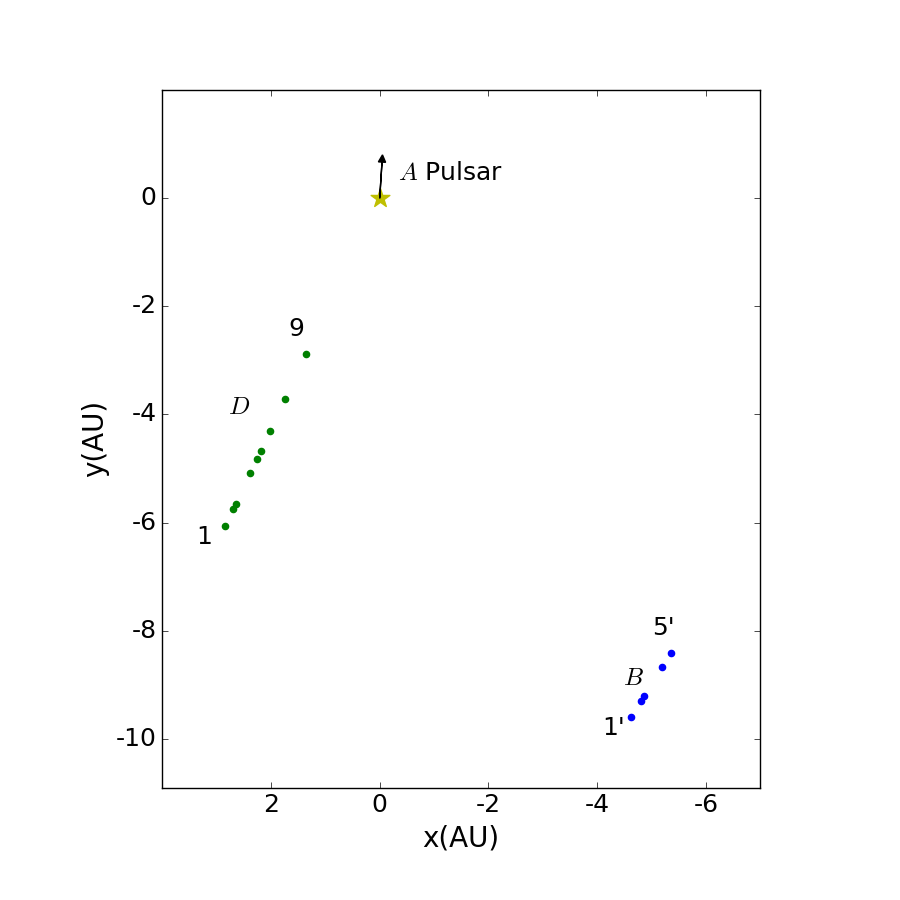
\includegraphics[width=0.7\textwidth]{Figures/Fig7_without_lines_5.png} 
}
\end{picture}
%\vspace{-4in}

  }

\frame{
    \frametitle{Lensing}
    \begin{itemize}
      \item observed on large scales in the ISM, outer scale $\sim 100$pc
      \item inner scale of $<1000$km proposed based on pulsar
        scintillation
      \item at odds with damping physics -- invoke undetermined plasma effects
      \item at odds with secondary spectra inverted parabolic arcs
        (Stinebring++ 2010++) and VLBI (Brisken et al 2010)
      \item intermittent, non-Gaussian, omni-predictive
      \item common misconception: pulsar scintillation is related to turbulence
    \end{itemize}

}


  \frame{
    \frametitle{Grazing incidence}
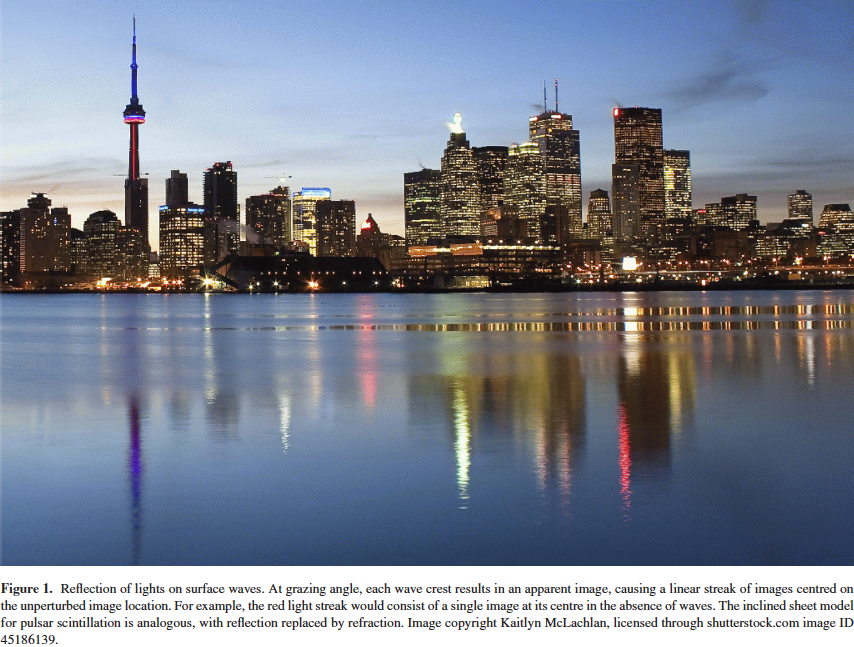
\includegraphics[width=0.9\textwidth]{Figures/toronto.png}
  }


\frame{
    \frametitle{Interference}
    \begin{itemize}
      \item Goldreich Sridhar 2006: refractive images generically
        interfere, e.g. double slit
      \item leads to scintillation scaling $\Delta \nu\propto \nu^{-4}$
      \item projected density caustics: Snell's law diverges
      \item statistics of alignment: rare alignments dominate
        lensing/scattering
      \item use ISM as giant billion km telescope!
    \end{itemize}
\tiny (from wikipedia)
\vspace{-0.05in}\hspace{2.55in}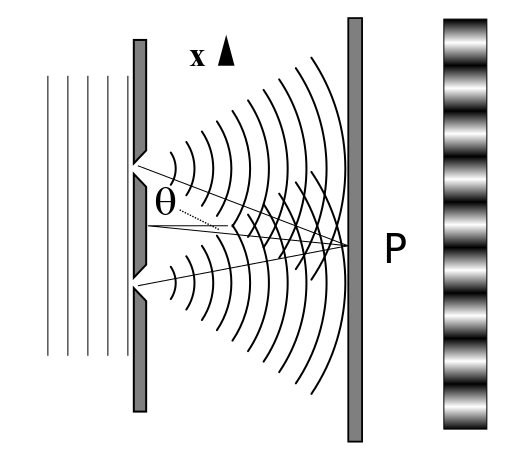
\includegraphics[width=0.4\textwidth]{Figures/Doubleslit.png}
}

  \frame{
    \frametitle{Current Sheets}
    \begin{itemize}
      \item magnetic field directional change is exact solution to MHD
        equilibrium: topological domain boundaries
      \item stability unknown, meta-stable (Sweet-Parker 1957+) or unstable (tearing
        mode, Petscheck 1964, +++)
      \item proposed as source of scattering (Goldreich-Sridhar 2006,
        Pen-Levin 2014)
    \end{itemize}
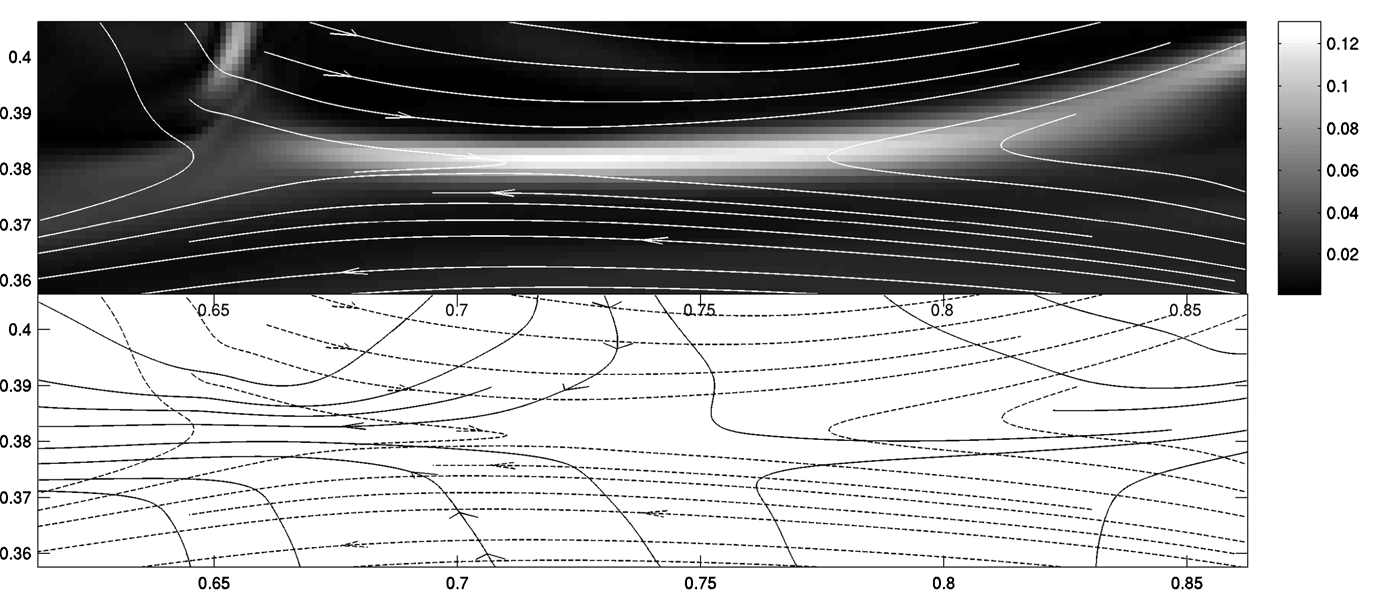
\includegraphics[width=0.9\textwidth]{Figures/reconnection.png} \tiny (Pang+2011)
  }

  \frame{
    \frametitle{Revisit}
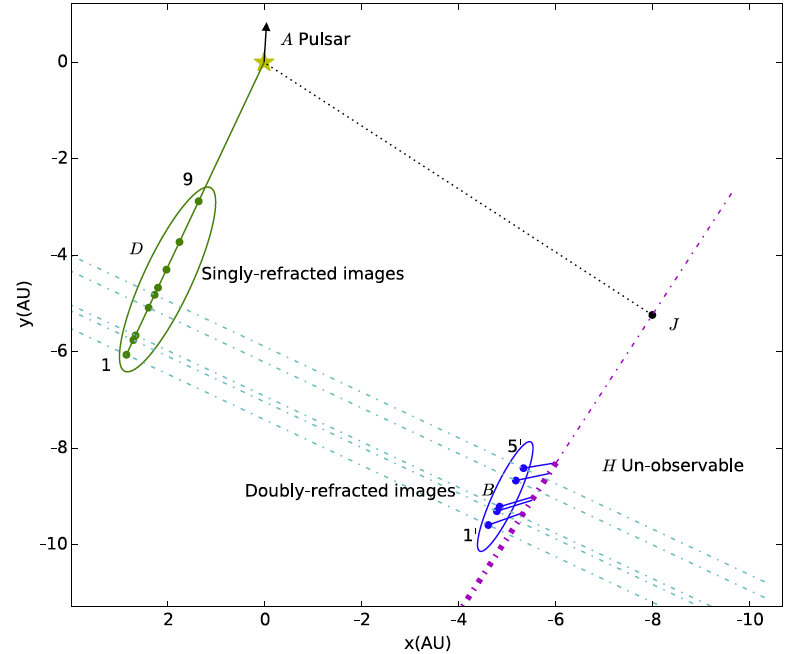
\includegraphics[width=0.8\textwidth]{Figures/liu-lens.png} \tiny
Brisken+2010, Liu+Pen 2016
  }



  \frame{
    \frametitle{Conclusion}
    \begin{itemize}
    \item Moon gives unique baselines to study ISM using pulsar
      propagation 
        \item access to low frequencies
      \item VLBI maps ISM plasma lenses
      \item ISM lenses map neighborhood microscopes
      \item potential to measure pulsar distances, ISM structure
    \end{itemize}
  }

\end{document}
